%!TEX root = ../../entwurfsprojekt2_entwurfsdokument.tex

\begin{figure}[h]
	\centering
	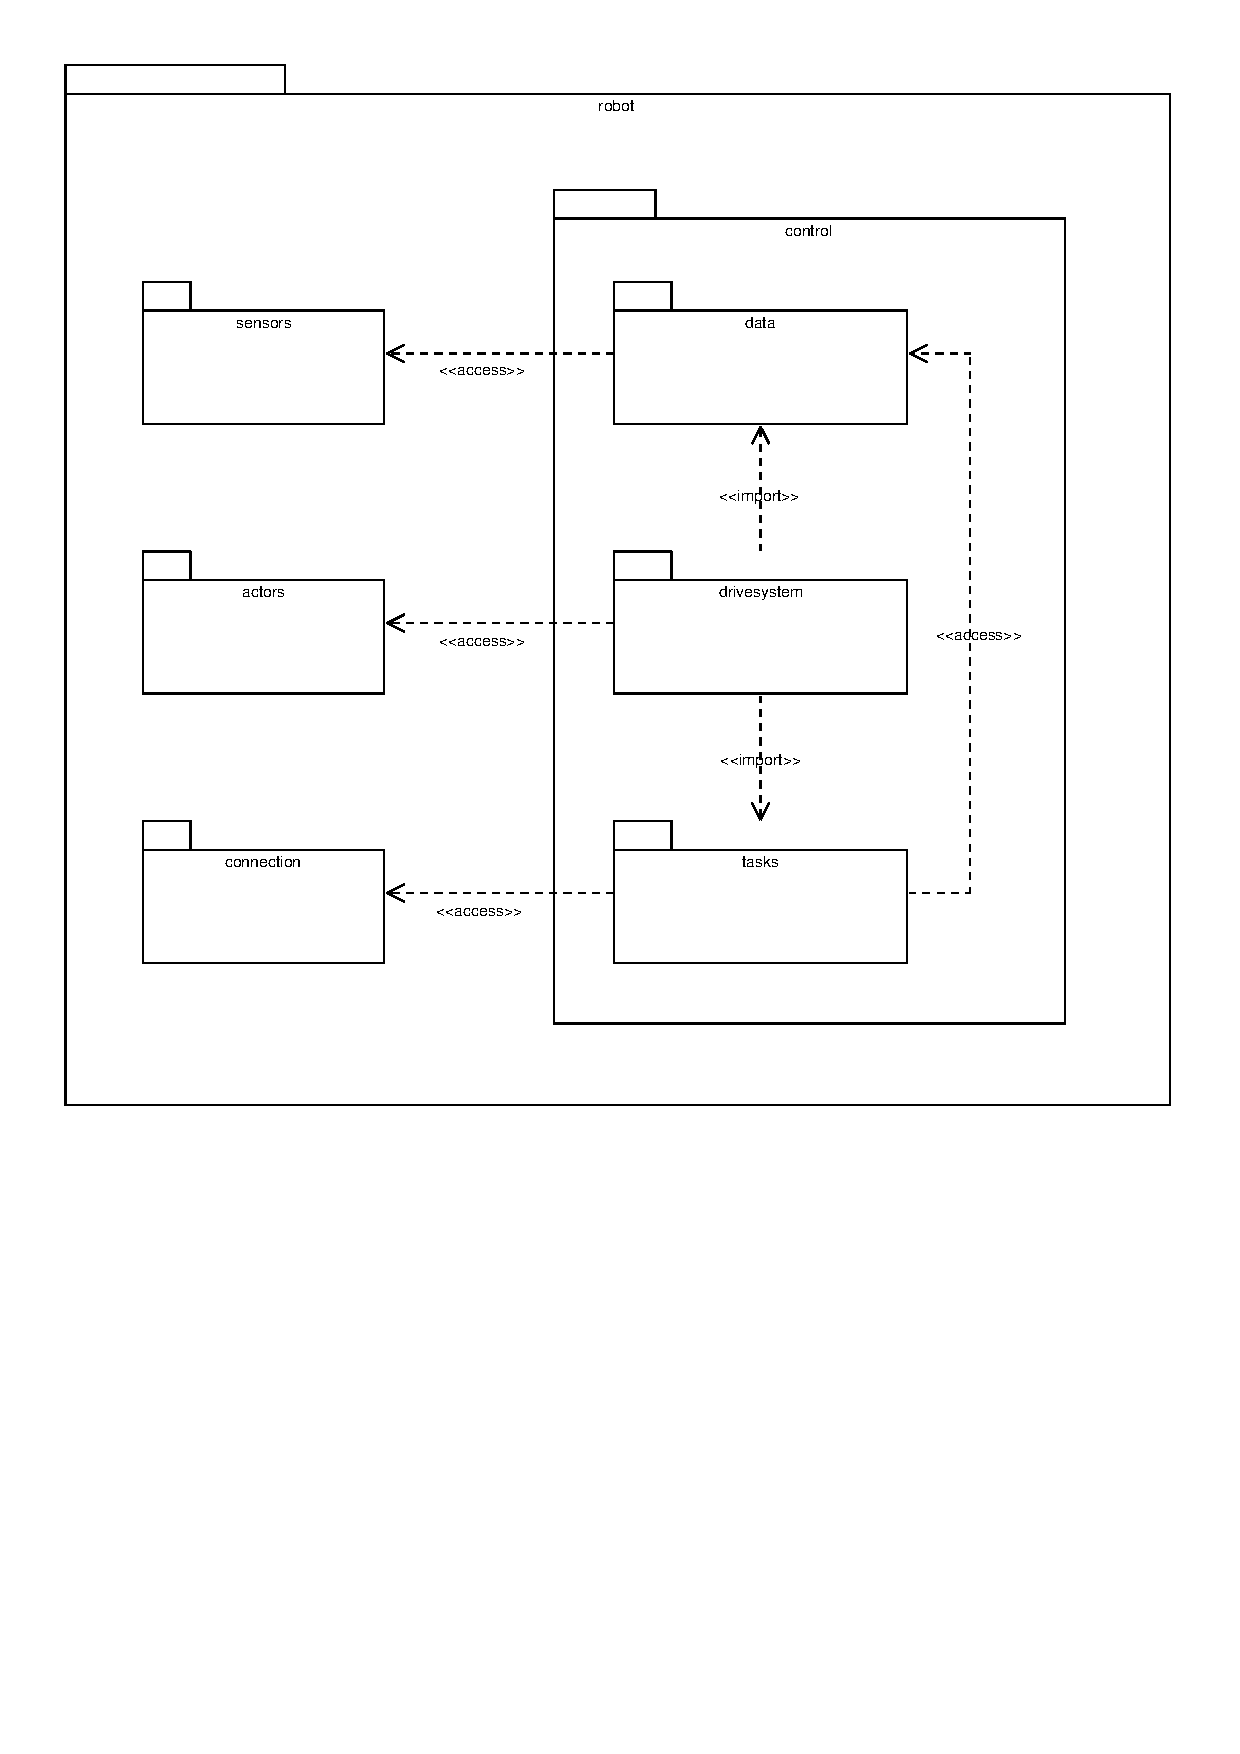
\includegraphics[width=0.7\textwidth]{robot_packages}
	\caption{Paketstruktur des Roboterteilsystems.}
	\label{fig:robot_packages}
\end{figure}

\section{Paketstruktur}
\label{sec:pakete}



Die Inhalte der Komponente \texttt{LogisticsRobot} werden in dem Paket \texttt{robot} implementiert.
Dieses enthält für jede der vier Unterkomponenten \texttt{RobotControl}, \texttt{RobotActors}, \texttt{RobotSensors} und \texttt{RobotNetwork} ein Unterpaket. 
Die Unterpakete \texttt{actors}, \texttt{sensors} und \texttt{connection} sind nicht weiter unterteilt, während das Unterpaket \texttt{control} noch einmal in die Unterpakete \texttt{data}, \texttt{drivesystem} und \texttt{tasks} aufgeteilt ist.

Die sich ergebende Paketstruktur mit den Abhängigkeiten zwischen den einzelnen Paketen ist in \autoref{fig:robot_packages} dargestellt.
